\section{Singleton}

O padrão Singleto fornece um ponto de acesso global a um objeto 
e garante que ele possuirá apenas uma instância. Esse padrão 
é importante para implementar serviços e oferecer acesso a eles
sem instanciar vários objetos iguais em diversos pontos diferentes 
do código.


\begin{figure}[htb]
	\caption{\label{singleton_struct}Estrutura do Singleton}
	\begin{center}
	    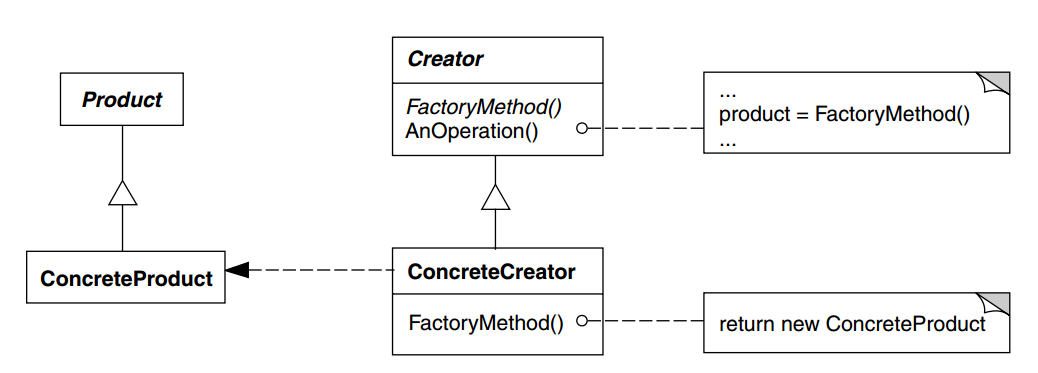
\includegraphics[scale=0.4]{5_padroes-contexto-funcional/5.1_criacionais/5.1.1_factory-method/diagram.png}
	\end{center}
\end{figure}

Exemplo Orientado a Objetos:

\begin{lstlisting}[caption={Singleton Orientação a Objetos},label=oosingleton]
    
    class Database private () {

        def query(sql)

    }

    object Database {

        private val _instance = new Database()
        def instance() = _instance

    }

\end{lstlisting}

Contexto Funcional:

Não existe uma forma de implementar o Singleton no contexto funcional 
por que ele viola o conceito de função pura, ou seja, a função não 
está mais dependendo apenas de seus parâmetros, mas também de um 
valor global que ainda pode ter seu estado modificado.

Porém, ainda existem formas de alcançar seu objetivo, ou seja, 
oferecer acesso a um serviço em diversos locais do código sem a necessidade 
de repeti-lo. A primeira forma é usando um conceito que não é exlusivamente funcional, 
já que até no contexto orientdo a objetos é considerado um bom substituto 
para o Singleton. Porém, por ser uma abordagem também utilizada por 
programas que seguem o paradigma funcional e consequentemente por não 
violar o paradigma, será mencionado como uma possível solução.

A abordagem consiste no uso da Injeção de Dependência, onde a criação de 
recurso utilizado por uma função ou objeto não é responsabilidade da mesma, 
ao invés disso, esse recurso é injetado, seja pelo construtor (no caso da 
orientação a objetos) ou por parâmetros de uma função (no caso do paradigma 
funcional).

\begin{lstlisting}[caption={Injeção de Dependência funcional},label=fpdi]
    
    

\end{lstlisting}

A segunda abordagem consiste na utilização de um Monad conhecido como 
Reader. As funções que precisam utilizar um determinado serviço são 
encapsuladas em um Monad. O estado desse serviço será acessável dentro 
dessas funções e sempre que suas execuções terminarem, o novo estado 
do serviço será retornado. Dessa forma, a próxima função que deseja 
utilizar o serviço poderá usufruir do estado atualizado.

\begin{lstlisting}[caption={Monad Reader},label=fpreader]
    
    

\end{lstlisting}

Essa abordagem tem algumas vantagens se comparada à injeção de dependência: 
Suponha que três funções são encadeadas em um programa. A primeira e a terceira 
precisarão utilizar o serviço que é injetado através dos parâmetros. A segunda 
função, mesmo sem utilizar o serviço, precisará recebê-lo em seus parâmetros 
para que ele seja passado para a terceira função. Isso diminui a reusabilidade 
dessa função, que poderia ser reaproveitada em um contexto onde o serviço não 
é necessário. Também há a poluição visual ao incluir, em diversas funções, 
parâmetros diferentes para fornecer os serviços. Em casos em que mais de um serviço 
é utilizado, a situação torna-se ainda mais caótica.